
\section[Phylogenetic Analysis by Maximum Likelihood (PAML)]{Phylogenetic Analysis by Maximum Likelihood (PAML)}
\label{sec:paml}
\addcontentsline{toc}{section}{\thesection. Phylogenetic Analysis by Maximum Likelihood (PAML)}

PAML~\citep{Yang1997,Yang2007} is one of the popular packages for estimating
phylogenetic trees given nucleotide, codon, or amino acid sequences. It searches
the optimal tree by maximum likelihood, and implements several different
options, models, algorithms and statistical tests to finding appropriate
trees which can interpreter the relations of sequences or species in an
evolutionary manner. The package contains several programs to perform
the phylogenetic analysis.
The original source code and documentation are available on the authors'
original website, or the mirror on phyloclustering website at
\url{https://snoweye.github.io/phyclust/}.

Among the programs, only \code{baseml} is ported into
\pkg{phyclust}, and the main function \code{paml.baseml()} in \proglang{R}
can find trees for nucleotide sequences.
Most of functionalities of \code{baseml} are transfered correctly, but I
disable some advance options due to complexity of input and output.
I also provide options for \code{paml.baseml()} to bridge the options of
\code{ms()}, \code{seqgen()}, and \code{phyclust()}.

The following Section~\ref{sec:pamlbaseml} introduces the usage of
\code{paml.baseml()} and it's control function.
Section~\ref{sec:phyclustpamlbaseml} illustrates examples for finding the
ancestral tree given central sequences of clusters.
This provides a two-stages approach to building a phylogeny on a large dataset,
and is an extension of Phyloclustering.




\subsection[Using the paml.baseml() function]{Using the \code{paml.baseml()} function}
\label{sec:pamlbaseml}
\addcontentsline{toc}{subsection}{\thesubsection. Using the \code{paml.baseml()}\ function}
 
The inputs of \code{baseml} relies on several files
including the tree file, sequence file, and control file. The outputs of \code{baseml}
are also several files depending on the controls.
The main function \code{paml.baseml()} is implemented in the same way of \code{ms()}
and \code{seqgen()}. The I/O design is to all store to and read from a temporary
directory which will be removed after computing is finish.
Use the following code to see the default controls and the details of the
main function.
\begin{Code}
> ?paml.baseml
> paml.baseml.show.default()
\end{Code}

The following example uses \code{paml.baseml()} to obtain the best tree
for the given model and to compare the best to the true tree. Here, we
only use a small data (five sequences) to test the program. Note that the
best is in terms of the highest likelihood of the given model
among a finite subset of tree space. This tree may or may not a good candidate
to interpreter the data. For a large dataset, it may take long time to find
the best tree.
\begin{Code}
> ### Generate data.
> set.seed(123)
> ret.ms <- ms(nsam = 5, nreps = 1, opts = "-T")
> ret.seqgen <- seqgen(opts = "-mHKY -l40 -s0.2", newick.tree = ret.ms[3])
> (ret.nucleotide <- read.seqgen(ret.seqgen))
code.type: NUCLEOTIDE, n.seq: 5, seq.len: 40, byrow: TRUE.
> X <- ret.nucleotide$org
> seqname <- ret.nucleotide$seqname
> 
> ### Run baseml.
> opts <- paml.baseml.control(model = 4, clock = 1)
> (ret.baseml <- paml.baseml(X, seqname = seqname, opts = opts))
((s1: 0.000000, s5: 0.000000): 0.091018, ((s2: 0.012639, s4: 0.012639): 0.02...
> (ret.baseml.init <- paml.baseml(X, seqname = seqname, opts = opts,
+    newick.trees = ret.ms[3]))
((s1: 0.000000, s5: 0.000000): 0.091018, ((s2: 0.012639, s4: 0.012639): 0.02...
> ret.ms[3]
[1] "((s1: 0.072680674493,s5: 0.072680674493): 0.498367525637,(s2: 0.1790905...
> 
> ### Unrooted tree.
> opts <- paml.baseml.control(model = 4)
> (ret.baseml.unrooted <- paml.baseml(X, seqname = seqname, opts = opts))
(((s1: 0.000004, s5: 0.000004): 0.141411, s2: 0.000004): 0.025586, s3: 0.052...
>
> par(mfrow = c(2, 2))
> plot(read.tree(text = ret.ms[3]), main = "true")
> plot(read.tree(text = ret.baseml$best.tree), main = "baseml")
> plot(read.tree(text = ret.baseml.init$best.tree),
>      main = "baseml with initial")
> plot(unroot(read.tree(text = ret.baseml.unrooted$best.tree)),
>      main = "baseml unrooted")
\end{Code}
\begin{figure}[h]
\begin{center}
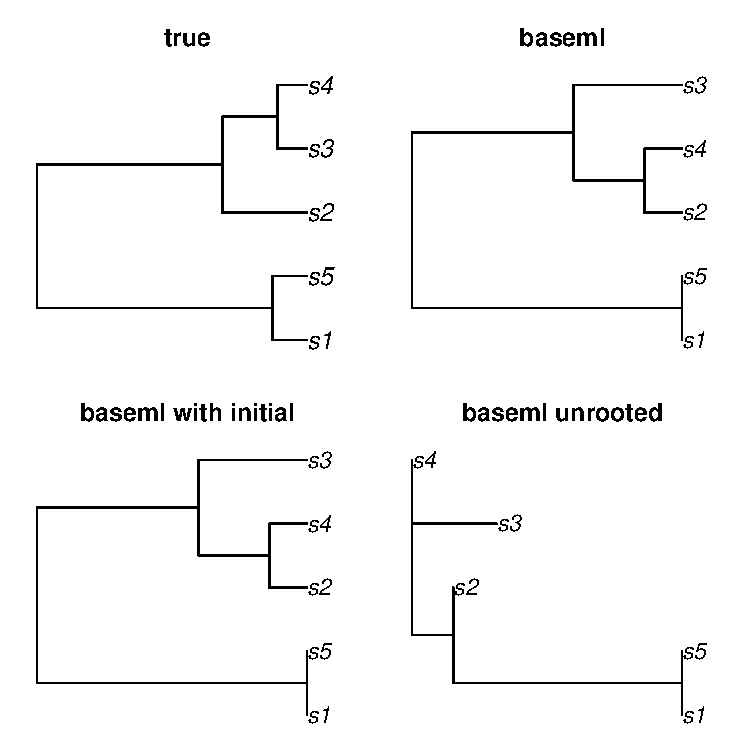
\includegraphics[width=5.0in]{./phyclust-include/f-paml_baseml}
\caption{A true tree and an estimation.}
\label{fig:pamlbaseml}
\end{center}
\end{figure}


The option \code{opts} of \code{paml.baseml()} will take a list
generated by \code{paml.baseml.control()} by default.
The output of \code{paml.baseml()} is also a list containing all files
as dumped by PAML. The element \code{mlb} contains the major results as
the option \code{outfile} specified by PAML. The element \code{stdout}
contains all STDOUT which is directly printed by PAML and is controlled by
the options \code{noisy} and \code{verbose}.
Note that due to the complexity of input and output, the multiple genes option
may be disable.

\begin{color}{red}Warning:\end{color}
The \code{ms()} generates an ultimate tree which is a rooted tree with
the same height to all leaves, but the PAML will search an unrooted tree by
default. PAML may also return a rooted tree for an unrooted tree with
multifurcation at the root.




\subsection[The phyclust+paml.baseml approach]{The phyclust+paml.baseml approach}
\label{sec:phyclustpamlbaseml}
\addcontentsline{toc}{subsection}{\thesubsection. The \code{phyclust+paml.baseml}\ approach \vspace{-0.3cm}}

For a large dataset,
it is a straight forward to consider the combination of the
\code{phyclust()} and \code{paml.baseml()} where Phyloclustering
find central sequences for populations and PAML find the phylogeny for
the central sequences. Similary to
the supertree~\citep{Bininda2004,Bininda2002},
this approach provides a different way of finding
phylogeny to the phylogenetic analysis. Note that the best number of
clusters and the best model for the phylogeny are all needed to be
determined, either by information criteria or by bootstrap.

The following is an interesting illustration for the toy dataset in
\pkg{phyclust} using \code{phyclust()} followed by \code{paml.baseml()}.
The Figure~\ref{fig:toynj} is the result for the same dataset
comparing to this Figure~\ref{fig:phyclustpamlbaseml},
while the former uses the distance approach and
the later uses the maximum likelihood approachs (Phyloclustering and PAML).
Note that the Figure~\ref{fig:phyclustpamlbaseml} has the same topology as
the true where the toy data genetated from.
\begin{Code}
> ### Fit a EE, JC69 model using emEM and fit an ancestral tree.
> EMC <- .EMControl(init.procedure = "emEM")
> set.seed(1234)
> K <- 4
> ret.K <- phyclust(seq.data.toy$org, K, EMC = EMC)
> (ret.Mu <- paml.baseml(ret.K$Mu, opts = paml.baseml.control()))
> tree.est <- read.tree(text = ret.Mu$best.tree)
> 
> ### Construct descent trees.
> for(k in 1:K){
>   tree.dec <- gen.star.tree(ret.K$n.class[k], total.height = ret.K$QA$Tt) 
>   tree.est <- bind.tree(tree.est, tree.dec,
>                           where = which(tree.est$tip.label == as.character(k)))
> }
> est.class <- rep(1:K, ret.K$n.class)
> plotnj(unroot(tree.est), X.class = est.class, main = "tree of sequences")
\end{Code}
\begin{figure}[h]
\begin{center}
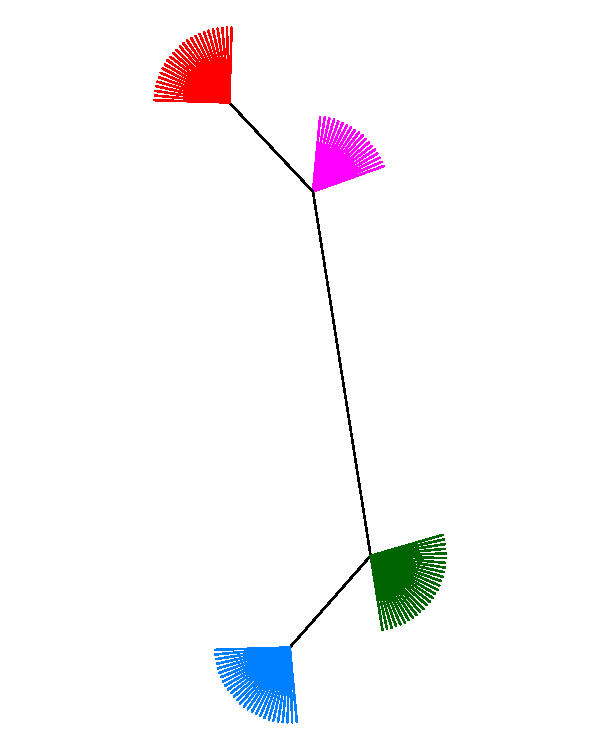
\includegraphics[width=4.0in]{./phyclust-include/f-super}
\caption{An estimation tree from \code{phyclust()} and \code{paml.baseml()}.}
\label{fig:phyclustpamlbaseml}
\end{center}
\end{figure}

